\documentclass{report}
\usepackage{graphicx, tikz-cd, float, titlepic, booktabs} % Required for inserting images
\usepackage{pgfplots}
\pgfplotsset{compat=1.15}
\usepackage{mathrsfs}
\usetikzlibrary{arrows}
\usepackage{amsmath, amssymb, amsthm, amsfonts, siunitx, physics, gensymb}
\AtBeginDocument{\RenewCommandCopy\qty\SI}
\usepackage[version=4]{mhchem}
\usepackage[most,many,breakable]{tcolorbox}
\usepackage{xcolor, fancyhdr, varwidth}
\usepackage[Glenn]{fncychap}
%Options: Sonny, Lenny, Glenn, Conny, Rejne, Bjarne, Bjornstrup
\usepackage{hyperref, cleveref}
\usepackage{icomma, enumitem} %comma as decimal and continue enumerate with [resume]
\usepackage{plimsoll} %use standard state symbol with \stst
\usepackage[danish]{babel}
%%%%%%%%%%%%%%%%%%%%%%%%%%%%%%
% SELF MADE COLORS
%%%%%%%%%%%%%%%%%%%%%%%%%%%%%%
\definecolor{myg}{RGB}{56, 140, 70}
\definecolor{myb}{RGB}{45, 111, 177}
\definecolor{myr}{RGB}{199, 68, 64}
\definecolor{mytheorembg}{HTML}{F2F2F9}
\definecolor{mytheoremfr}{HTML}{00007B}
\definecolor{mylenmabg}{HTML}{FFFAF8}
\definecolor{mylenmafr}{HTML}{983b0f}
\definecolor{mypropbg}{HTML}{f2fbfc}
\definecolor{mypropfr}{HTML}{191971}
\definecolor{myexamplebg}{HTML}{F2FBF8}
\definecolor{myexamplefr}{HTML}{88D6D1}
\definecolor{myexampleti}{HTML}{2A7F7F}
\definecolor{mydefinitbg}{HTML}{E5E5FF}
\definecolor{mydefinitfr}{HTML}{3F3FA3}
\definecolor{notesgreen}{RGB}{0,162,0}
\definecolor{myp}{RGB}{197, 92, 212}
\definecolor{mygr}{HTML}{2C3338}
\definecolor{myred}{RGB}{127,0,0}
\definecolor{myyellow}{RGB}{169,121,69}
\definecolor{myexercisebg}{HTML}{F2FBF8}
\definecolor{myexercisefg}{HTML}{88D6D1}
%%%%%%%%%%%%%%%%%%%%%%%%%%%%%%%%%%%%%%%%%%%%%%%%%%%%%%%%%%%%%%%%%%%%%%
% Box environments for theorems and problems
%%%%%%%%%%%%%%%%%%%%%%%%%%%%%%%%%%%%%%%%%%%%%%%%%%%%%%%%%%%%%%%%%%%%%
\setlength{\parindent}{1cm}
%================================
% Question BOX
%================================
\makeatletter
\newtcbtheorem{question}{Opgave}{enhanced,
	breakable,
	colback=white,
	colframe=myb!80!black,
	attach boxed title to top left={yshift*=-\tcboxedtitleheight},
	fonttitle=\bfseries,
	title={#2},
	boxed title size=title,
	boxed title style={%
			sharp corners,
			rounded corners=northwest,
			colback=tcbcolframe,
			boxrule=0pt,
		},
	underlay boxed title={%
			\path[fill=tcbcolframe] (title.south west)--(title.south east)
			to[out=0, in=180] ([xshift=5mm]title.east)--
			(title.center-|frame.east)
			[rounded corners=\kvtcb@arc] |-
			(frame.north) -| cycle;
		},
	#1
}{def}
\makeatother
%================================
% DEFINITION BOX
%================================

\newtcbtheorem[]{Definition}{Definition}{enhanced,
	before skip=2mm,after skip=2mm, colback=red!5,colframe=red!80!black,boxrule=0.5mm,
	attach boxed title to top left={xshift=1cm,yshift*=1mm-\tcboxedtitleheight}, varwidth boxed title*=-3cm,
	boxed title style={frame code={
					\path[fill=tcbcolback]
					([yshift=-1mm,xshift=-1mm]frame.north west)
					arc[start angle=0,end angle=180,radius=1mm]
					([yshift=-1mm,xshift=1mm]frame.north east)
					arc[start angle=180,end angle=0,radius=1mm];
					\path[left color=tcbcolback!60!black,right color=tcbcolback!60!black,
						middle color=tcbcolback!80!black]
					([xshift=-2mm]frame.north west) -- ([xshift=2mm]frame.north east)
					[rounded corners=1mm]-- ([xshift=1mm,yshift=-1mm]frame.north east)
					-- (frame.south east) -- (frame.south west)
					-- ([xshift=-1mm,yshift=-1mm]frame.north west)
					[sharp corners]-- cycle;
				},interior engine=empty,
		},
	fonttitle=\bfseries,
	title={#2},#1}{def}
\newtcbtheorem[]{definition}{Definition}{enhanced,
	before skip=2mm,after skip=2mm, colback=red!5,colframe=red!80!black,boxrule=0.5mm,
	attach boxed title to top left={xshift=1cm,yshift*=1mm-\tcboxedtitleheight}, varwidth boxed title*=-3cm,
	boxed title style={frame code={
					\path[fill=tcbcolback]
					([yshift=-1mm,xshift=-1mm]frame.north west)
					arc[start angle=0,end angle=180,radius=1mm]
					([yshift=-1mm,xshift=1mm]frame.north east)
					arc[start angle=180,end angle=0,radius=1mm];
					\path[left color=tcbcolback!60!black,right color=tcbcolback!60!black,
						middle color=tcbcolback!80!black]
					([xshift=-2mm]frame.north west) -- ([xshift=2mm]frame.north east)
					[rounded corners=1mm]-- ([xshift=1mm,yshift=-1mm]frame.north east)
					-- (frame.south east) -- (frame.south west)
					-- ([xshift=-1mm,yshift=-1mm]frame.north west)
					[sharp corners]-- cycle;
				},interior engine=empty,
		},
	fonttitle=\bfseries,
	title={#2},#1}{def}

\newtcbtheorem{theo}%
    {Theorem}{}{theorem}
\newtcolorbox{prob}[1]{colback=red!5!white,colframe=red!50!black,fonttitle=\bfseries,title={#1}}
%================================
% NOTE BOX
%================================

\usetikzlibrary{arrows,calc,shadows.blur}
\tcbuselibrary{skins}
\newtcolorbox{note}[1][]{%
	enhanced jigsaw,
	colback=gray!20!white,%
	colframe=gray!80!black,
	size=small,
	boxrule=1pt,
	title=\textbf{Note:},
	halign title=flush center,
	coltitle=black,
	breakable,
	drop shadow=black!50!white,
	attach boxed title to top left={xshift=1cm,yshift=-\tcboxedtitleheight/2,yshifttext=-\tcboxedtitleheight/2},
	minipage boxed title=1.5cm,
	boxed title style={%
			colback=white,
			size=fbox,
			boxrule=1pt,
			boxsep=2pt,
			underlay={%
					\coordinate (dotA) at ($(interior.west) + (-0.5pt,0)$);
					\coordinate (dotB) at ($(interior.east) + (0.5pt,0)$);
					\begin{scope}
						\clip (interior.north west) rectangle ([xshift=3ex]interior.east);
						\filldraw [white, blur shadow={shadow opacity=60, shadow yshift=-.75ex}, rounded corners=2pt] (interior.north west) rectangle (interior.south east);
					\end{scope}
					\begin{scope}[gray!80!black]
						\fill (dotA) circle (2pt);
						\fill (dotB) circle (2pt);
					\end{scope}
				},
		},
	#1,
}
%================================
% EXAMPLE BOX
%================================
\newtcbtheorem[number within=section]{Example}{Example}
{%
	colback = myexamplebg
	,breakable
	,colframe = myexamplefr
	,coltitle = myexampleti
	,boxrule = 1pt
	,sharp corners
	,detach title
	,before upper=\tcbtitle\par\smallskip
	,fonttitle = \bfseries
	,description font = \mdseries
	,separator sign none
	,description delimiters parenthesis
}
{ex}
%================================
% THEOREM BOX
%================================

\tcbuselibrary{theorems,skins,hooks}
\newtcbtheorem[number within=section]{Theorem}{Theorem}
{%
	enhanced,
	breakable,
	colback = mytheorembg,
	frame hidden,
	boxrule = 0sp,
	borderline west = {2pt}{0pt}{mytheoremfr},
	sharp corners,
	detach title,
	before upper = \tcbtitle\par\smallskip,
	coltitle = mytheoremfr,
	fonttitle = \bfseries\sffamily,
	description font = \mdseries,
	separator sign none,
	segmentation style={solid, mytheoremfr},
}
{th}

%%%%%%%%%%%%%%%%%%%%%%%%%%%%%%%%%%%%%%%%%%%%%%%%%%%%%%%%%%%%%%%%%
% SELF MADE COMMANDS
%%%%%%%%%%%%%%%%%%%%%%%%%%%%%%
\newcommand{\sol}{\setlength{\parindent}{0cm}\textbf{\textit{Løsning:}}\setlength{\parindent}{1cm}}
%%%%%%%%%%%%%%%%%%%%%%%%%%%%%%%%%
\usepackage[tmargin=2cm,rmargin=1in,lmargin=1in,margin=0.85in,bmargin=2cm,footskip=.2in]{geometry}\pagestyle{fancy}
\lhead{Minrui Kevin Zhou 3.b}
\rhead{H5}

\title{H5\\
{\Large \textbf{3.b fysik A}}}
\author{Kevin Zhou}
\date{\today}

\begin{document}
\maketitle
\begin{question}{Lysende halsbånd}{}
  Et kredsløb i et hundehalsbånd med lysdioder indeholder en resistor $R$ med resistansen 5,00 $\Omega$. Den maksimale effekt, hvormed der må afsættes energi i resistoren, er 0,25 W.
  \begin{itemize}
    \item[a.] Beregn strømstyrken igennem resistoren, når den afsatte effekt er maksimal
  \end{itemize}
Resistoren sidder i et kredsløb med seks ens lysdioder og et batteri som vist i diagrammet.
Grafen viser, hvordan strømstyrken $I$ gennem en lysdiode afhænger af spændingsfaldet $U_\mathrm{lysdiode}$ over den.
Når hundehalsbåndet Iyser, er spændingsfaldet over lysdioderne 2,72 V.
\begin{itemize}
  \item[b.] Bestem spændingsfaldet $U$ over batteriet, når hundehalsbåndet lyser.
\end{itemize}
\end{question}
\sol \\
\textbf{a.}
Da der er tale om en resistor, så gælder Ohms lov:
\[
U=R \cdot I
\] 
Der gælder for effekten, hvormed der omsættes elektrisk energi i resistoren, at
\begin{equation*}
\begin{split}
  P=U \cdot I &\implies P=R \cdot I^2 \\
  &\iff I=\sqrt{\frac{P}{R}} 
\end{split}
\end{equation*}
da $I$ må være en positiv størrelse.
Vi beregner nu strømstyrken.
\begin{equation*}
\begin{split}
  I&=\sqrt{\frac{P}{R}} \\
  &=\sqrt{\frac{0,25 \;\unit{W} }{5,00 \;\unit{\ohm} }} \\
  &\approx 0,22 \;\unit{A} 
\end{split}
\end{equation*}
Når den afsatte effekt er maksimal, så er strømstyrken gennem resistoren altså $0,22 \;\unit{A} $.\\[1ex]
\textbf{b.}
For lysdioderne i parallelforbindelse gælder der, at deres samlede spændingsfald må være spændningsfaldet for én diode.
Altså har vi 
\[
U_{\text{dioder samlet} }=U_{\text{lysdiode} }
\] 
Det aflæses på grafen, at når $U _{\text{lysdiode} }=2,72 \;\unit{V} $, så er $I_{\text{lysdiode} }=1,20 \;\unit{mA} $ (se \cref{fig:IU}).
\begin{figure}[H]
\begin{center}
  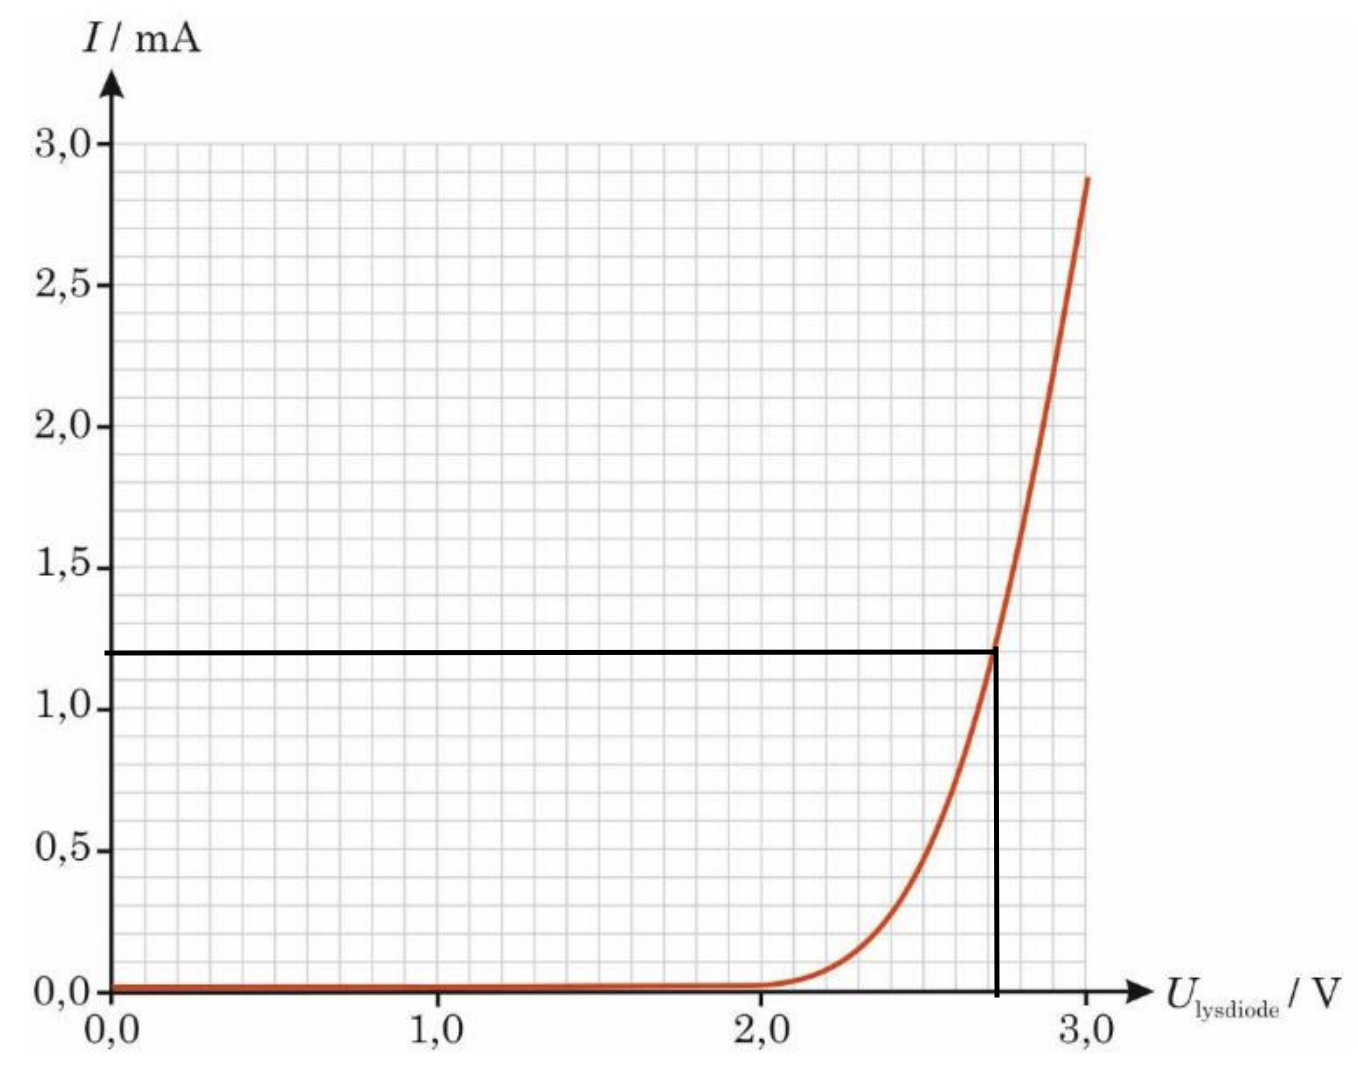
\includegraphics[scale=0.35]{IU.png}
\end{center}
\caption{Aflæsning på grafen}
\label{fig:IU}
\end{figure}

Siden lysdioderne sidder i parallelforbindelse, så må der gælde, at deres samlede strømstyrke må være summen af dem hver især:
\[
I=6 \cdot I_{\text{lysdiode} }
\] 
Da dioderne sidder i serie med resistoren, så må det være strømstyrken der løber i hele kredsløbet.

Da dioderne sidder i serie med resistoren, så må spændingsfaldet over batteriet være summen af resistorens spændingsfald og diodernes spændingsfald:
\begin{equation*}
\begin{split}
  U&=U_{\text{resistor} }+U_{\text{dioder samlet} }\\
  &=R_{\text{resistor} } \cdot I + U_{\text{lysdiode} }\\
  &=R_{\text{resistor} } \cdot 6 \cdot I_{\text{lysdiode} } + U_{\text{lysdiode} }\\
  &=5,00 \;\unit{\ohm} \cdot 6 \cdot 1,20 \cdot 10 ^{-3} \;\unit{A} + 2,72 \;\unit{V} \\
  &\approx 2,76 \;\unit{V}  
\end{split}
\end{equation*}
Når halsbåndet lyser, er spændingsfaldet over batteriet altså $2,76 \;\unit{V} $.

\begin{question}{Sort hul}{}
I visse tilfælde kan et sort hul opdages, ved at en stjerne i nærheden udfører en jævn cirkelbevægelse om det sorte hul. I 1992 undersøgte man ved hjælp af WATCH en sådan stjerne. Stjernes omløbstid er 10,4 timer, og farten i cirkelbevægelsen er $4,1 \cdot 10^5 \;\unit{m/s} $.
\begin{itemize}
  \item[a.] Beregn radius i cirkelbevægelsen
  \item[b.] Beregn massen af det sorte hul.
\end{itemize}
Jorden befinder sig i cirkelbevægelsens plan. Grafen viser, hvordan stjernens hastighed $v$ i forhold til Jorden varierer som funktion af tiden $t$. Hastigheden er målt langs sigtelinjen til stjernen. Hastigheden er positiv, når stjernen bevæger sig mod Jorden, mens den er negativ, når den bevæger sig væk fra Jorden.
\begin{itemize}
  \item[c.] 
Argumentér ved hjælp af grafen for, at farten i cirkelbevægelsen er $4,1 \cdot  10^{5} \;\unit{m/s} $. Bestem den fart, hvormed det sorte hul bevæger sig mod Jorden. 
\end{itemize}
\end{question}
\sol \\
\textbf{a.}
Da det er en jævn cirkelbevægelse gælder der, at 
\begin{equation*}
\begin{split}
  v=\frac{2 \pi \cdot r}{T} \iff r=\frac{v \cdot T}{2 \pi }
\end{split}
\end{equation*}
hvor $T$ er omløbstiden. 
Vi beregner nu radius 
\begin{equation*}
\begin{split}
  r&=\frac{v \cdot T}{2 \pi }\\
  &=\frac{4,1 \cdot 10^5 \;\unit{m/s} \cdot 10,4 \cdot 3600 \;\unit{s} }{2 \pi }\\
  &\approx 2,4 \cdot 10^9 \;\unit{m} \\
  &=2,4 \cdot 10^6 \;\unit{km} 
\end{split}
\end{equation*}
Altså er radius i cirkelbevægelsen $2,4 \cdot 10^6 \;\unit{km} $. \\[1ex]
\textbf{b.}
Siden stjernen ikke flyver ud eller bliver trukket ind, så må der gælde, at summen af dens kinetiske og potentielle energi fra gravitationsfeltet må være $0$:
\begin{equation*}
\begin{split}
  E_{\text{kin} }+E _{\text{pot} } &\iff \frac{1}{2} \cdot m_{\text{stjerne} } \cdot v^2 - G \cdot \frac{m_{\text{stjerne} } \cdot M _{\text{sort hul} }}{r}=0\\
  &\iff \frac{G}{r} \cdot M _{\text{sort hul} }=\frac{v^2}{2}\\
  &\iff M _{\text{sort hul} }= \frac{v^2 \cdot r}{2 \cdot G}
\end{split}
\end{equation*}
Vi beregner nu massen af det sorte hul.
\begin{equation*}
\begin{split}
  M _{\text{sort hul} }&= \frac{v^2 \cdot r}{2 \cdot G}\\
  &=\frac{\left(4,1 \cdot 10^5 \;\unit{m/s} \right)^2 \cdot 2,44309 \cdot 10^9 \;\unit{m} }{2 \cdot 6,674 \cdot 10 ^{-11}\;\unit{\frac{N \cdot m^2}{kg^2}} }\\
  &\approx 3,1 \cdot 10 ^{30} \;\unit{kg} 
\end{split}
\end{equation*}
Altså er massen af det sorte hul $3,1 \cdot 10^{30} \;\unit{kg} $. \\[1ex]
\textbf{c.}
Siden stjernen blot bevæger sig rundt om det sorte hul, og ikke kommer tættere på eller længere fra hullet, og stjernens fart er konstant, så må $(t,v)$-grafen være en vertikalt forskudt sinusbølge (fordi det sorte hul bevæger sig ift. jorden), og grafens amplitude må være farten for stjernen i cirkelbevægelsen.
Det aflæses på grafen (se gule markeringer i \cref{fig:tv}), at amplituden og farten i cirkelbevægelsen er 
\[
410 \;\unit{km/s} = 4,1 \cdot 10^2 \cdot 10^3 \;\unit{m/s} =4,1 \cdot 10^5\;\unit{m/s} 
\] 
Det sorte huls fart mod jorden må være forskellen mellem stjernens største og mindste fart mht. jorden, hvilket svarer til bølgens vertikale forskydning.
Denne aflæses (se \cref{fig:tv}) til at være $50 \;\unit{km/s} $.
Altså bevæger det sorte hul sig mod jorden med farten $50 \;\unit{km/s} $.

\begin{figure}[H]
\begin{center}
  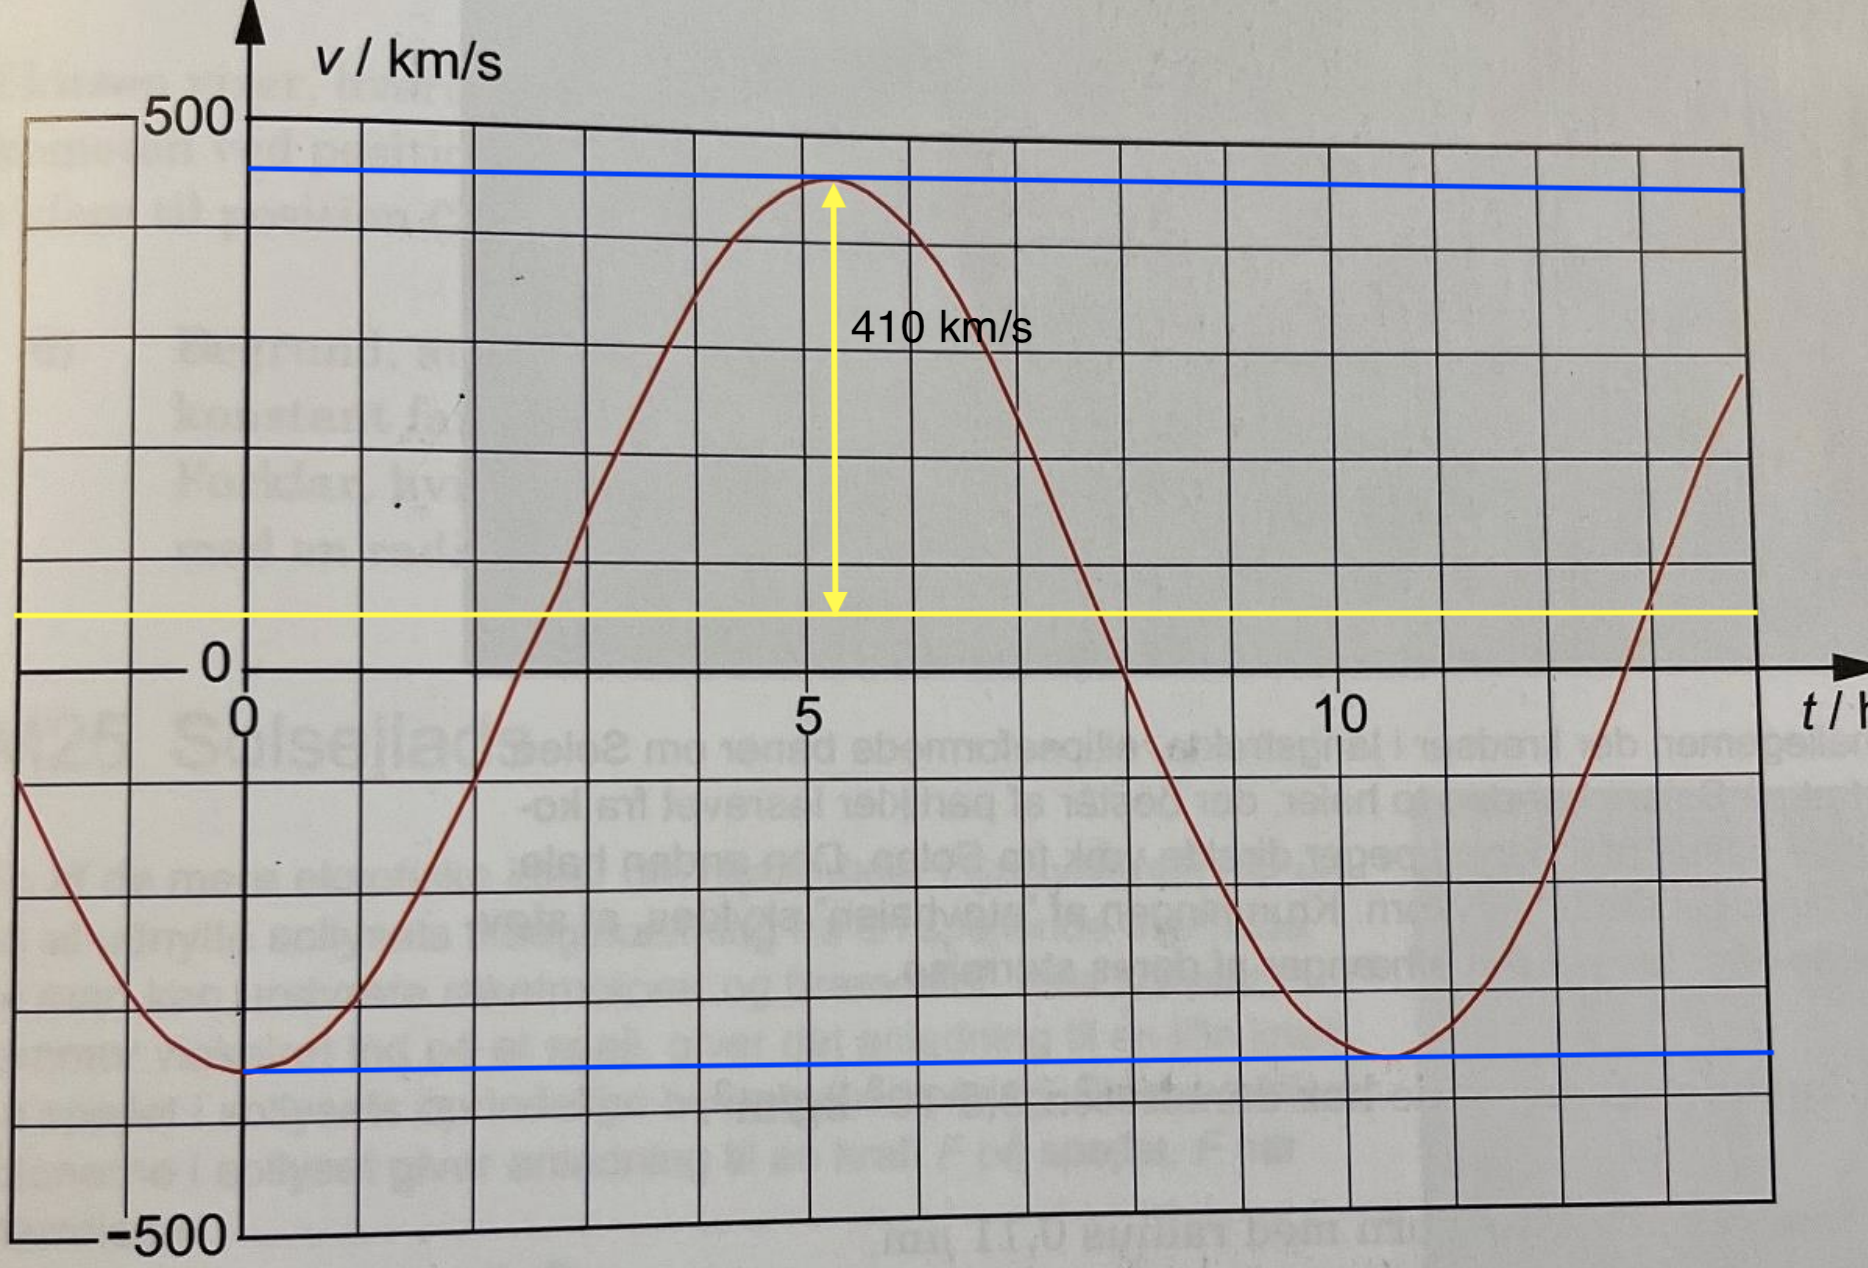
\includegraphics[scale=0.5]{vt.png}
\end{center}
  \caption{Aflæsning på $(t,v)$-grafen}
\label{fig:tv}
\end{figure}

\begin{question}{Solsejl}{}
  
\end{question}
\sol \\
\textbf{a.}
Vi finder først et udtryk for effekten af strålingsenergien $P$ udtrykt med hensyn til strålingsintensiteten $I$. 
\begin{equation*}
\begin{split}
  I=\frac{P}{A} \iff P=I \cdot A
\end{split}
\end{equation*}
Vi beregner størrelsen af kraften med den givne formel i opgavebeskrivelsen.
\begin{equation*}
\begin{split}
  F&=\frac{2 \cdot P}{c}\\
  &=\frac{2 \cdot I \cdot A}{c}\\
  &=\frac{2 \cdot 1370 \;\unit{W/m^2} \cdot 1,00 \;\unit{m^2} }{3,00 \cdot 10^8 \;\unit{m/s} }\\
  &\approx 9,13 \cdot 10 ^{-6} \;\unit{N} 
\end{split}
\end{equation*}
Altså er størrelsen af kraften fra solstrålingen, som rammer vinkelret ind på $1,00 \;\unit{m^2} $ af et solsejl i jordens afstand fra solen $9,13 \cdot 10 ^{-6} \;\unit{N}  $. \\[1ex]
\textbf{b.}
Størrelsen af kraften fra strålingen og størrelsen af gravitationskraften må være ens.
\begin{equation*}
\begin{split}
  F _{\text{stråling} }= F_G &\iff \frac{2 \cdot I \cdot A}{c}=G \cdot \frac{m_{\text{skib} }\cdot M _{\text{sol} }}{r^2}\\
  &\iff A=G \cdot \frac{m_{\text{skib} }\cdot M _{\text{sol} } \cdot c}{r^2 \cdot 2 \cdot I}
\end{split}
\end{equation*}
Vi kan nu beregne sejlarealet.
\begin{equation*}
\begin{split}
  A&=G \cdot \frac{m_{\text{skib} }\cdot M _{\text{sol} } \cdot c}{r^2 \cdot 2 \cdot I}\\
  &=6,674 \cdot 10 ^{-11}\;\unit{\frac{N \cdot m^2}{kg^2}} \cdot \frac{900 \;\unit{kg} \cdot 1,989 \cdot 10^{30} \;\unit{kg} \cdot 3,00 \cdot 10^8 \;\unit{m/s} }{(1,496 \cdot 10 ^{11} \;\unit{m})^2 \cdot 2 \cdot 1370 \;\unit{W/m^2} }\\
  &\approx  5,78 \cdot 10^5\;\unit{m^2} 
\end{split}
\end{equation*}
Altså skal sejlarealet være $ 5,78 \cdot 10^5\;\unit{m^2} $, for at kraftpåvirkningen fra solstrålingen lige netop kan holde ligevægt med gravitationskraften fra Solen.\\[1ex]
\textbf{c.}
Da gravitationskraften fra solen er modsatrettet strålingskraften, så må den størrelsen af den resulterende kraft i solstrålingens retning være
\begin{equation*}
\begin{split}
  F _{\text{res} }=F _{\text{stråling} }-F_G=m_{\text{skib} } \cdot a &\iff a=\frac{F _{\text{stråling} }-F_G}{m_{\text{skib} }}\\
  &\iff a=\frac{2 \cdot I \cdot A}{c \cdot m_{\text{skib} }}-G \cdot \frac{m_{\text{skib} }\cdot M _{\text{sol} }}{r^2\cdot m_{\text{skib} }}\\
  &\iff a=\frac{2 \cdot I \cdot A}{c \cdot m_{\text{skib} }} - G \cdot \frac{M_{\text{sol }}}{r^2}
\end{split}
\end{equation*}
Vi beregner nu rumskibets acceleration når det starter.
\begin{equation*}
\begin{split}
  a_0&=\frac{2 \cdot I \cdot A}{c \cdot m_{\text{skib} }} - G \cdot \frac{M_{\text{sol }}}{r^2}\\
  &=\frac{2 \cdot 1370 \;\unit{W/m^2} \cdot 1,20 \cdot 10^6 \;\unit{m^2} }{3,00 \cdot 10^8 \;\unit{m/s} \cdot 900 \;\unit{kg} } - 6,674 \cdot 10 ^{-11} \;\unit{\frac{N \cdot m^2}{kg^2}} \cdot \frac{1,989 \cdot 10 ^{30} \;\unit{kg} }{(1,496 \cdot 10 ^{11} \;\unit{m})^2 }\\
  &\approx 6,25 \cdot 10 ^{-3} \;\unit{m/s^2} 
\end{split}
\end{equation*}
Altså er skibets acceleration til start $6,25 \cdot 10 ^{-3} \;\unit{m/s} $.

Vi antager nu, at størrelsen af $F _{\text{stråling} }-F_G$ forholder sig konstant i første døgn, og at ingen andre kræfter påvirker skibet. 
Da er der tale om en konstant accelereret bevægelse, og siden bevægelsen var fra hvile, så må der gælde, at afstanden bliver 
\begin{equation*}
\begin{split}
  s&=\frac{1}{2} \cdot a \cdot t^2\\
  &=\frac{1}{2} \cdot 6,24637 \cdot 10^{-3} \;\unit{m/s^2} \cdot \left(24 \cdot 60^2 \;\unit{s} \right)^2 \\
  &\approx 2,33 \cdot 10^7\;\unit{m} 
\end{split}
\end{equation*}
I løbet af første døgn kan skibet altså tilbagelægge omkring $2,33 \cdot 10^7 \;\unit{m} $.\\[1ex]
\textbf{d.}
Energien som én foton leverer til solsejlet må være
\begin{equation*}
\begin{split}
  E_{\text{foton} }&=\frac{h \cdot c}{\lambda }
\end{split}
\end{equation*}
Vi kan nu udregne antallet af fotoner, der rammer sejlet på ét sekund, når det er i jordens afstand fra solen. 
Denne er blot forholdet mellem den samlede energi fra fotoner på et sekund samt energien fra én foton:
\begin{equation*}
\begin{split}
  \text{Antal} &=\frac{E_{\text{fotoner samlet} }}{E_{\text{foton} }}\\
  &=\frac{I \cdot A \cdot \Delta t}{\frac{h \cdot c}{\lambda }}\\
  &=\frac{I \cdot A \cdot \Delta t \cdot \lambda }{h \cdot c}\\
  &=\frac{1370 \;\unit{W/m^2} \cdot 1,20 \cdot 10^6 \;\unit{m^2} \cdot 1 \;\unit{s} \cdot 550 \cdot 10 ^{-9}\;\unit{m} }{6,6261 \cdot 10 ^{-34} \;\unit{J \cdot s} }\\
  &\approx 1,36 \cdot 10 ^{36} 
\end{split}
\end{equation*}
Når rumskibet starter, rammer $1,36 \cdot 10 ^{36}$ fotoner altså sejlet hvert sekund. 

Vi vil nu udlede formlen fra opgavebeskrivelsen.
Fra impulssætningen har vi, at 
\begin{equation*}
\begin{split}
  \Delta p_{\text{fot} }=F \cdot \Delta t &\iff F=\frac{\Delta p_{\text{fot} }}{\Delta t}\\
\end{split}
\end{equation*}
Ved refleksion gælder der for tilvæksten af bevægelsesmængde, at 
\begin{equation*}
\begin{split}
  \Delta p_{\text{fot} }&=p _{\text{fot,efter} }-p _{\text{fot,før} }\\
  &=p _{\text{fot,efter} }+p _{\text{fot,efter} }\\
  &=2 \cdot p _{\text{fot,efter} }
\end{split}
\end{equation*}
Ved at sætte de to udtryk sammen, får vi 
\begin{equation*}
\begin{split}
  F&=\frac{\Delta p_{\text{fot} }}{\Delta t}\\
  &=\frac{2 \cdot p _{\text{fot,efter} }}{\Delta t}\\
  &=\frac{2 \cdot h \cdot f}{ c\cdot \Delta t}\\
  &=\frac{2 }{c } \cdot \frac{ E _{\text{fot} }}{ \Delta t}\\
  &=\frac{2 \cdot P}{c}
\end{split}
\end{equation*}
hvilket var, hvad vi skulle vise.

\end{document}
